\section{Trådhåndtering}
For at effektivisere systemet anvendes tråde til håndtering af forskellige opgaver. Der anvendes en tråd til at styre den overordnede brugerflade, en til at styre regulering af systemet, en til monitorering af klimaet i drivhuset samt en til at håndtere system loggen. Ved at bruge tråde kan alle disse funktionaliteter køres parallelt. Dette giver en højere hastighed i systemet da funktionerne ikke skal vente på hinandens eksekvering. På Figur \ref{fig:SD_Threads} er der en visuel beskrivelse af disse tråde. Yderligere beskrivelse af tråde kan findes under literaturliste \cite{lib:threadconcept}.

\begin{figure}[!h]
\centering 
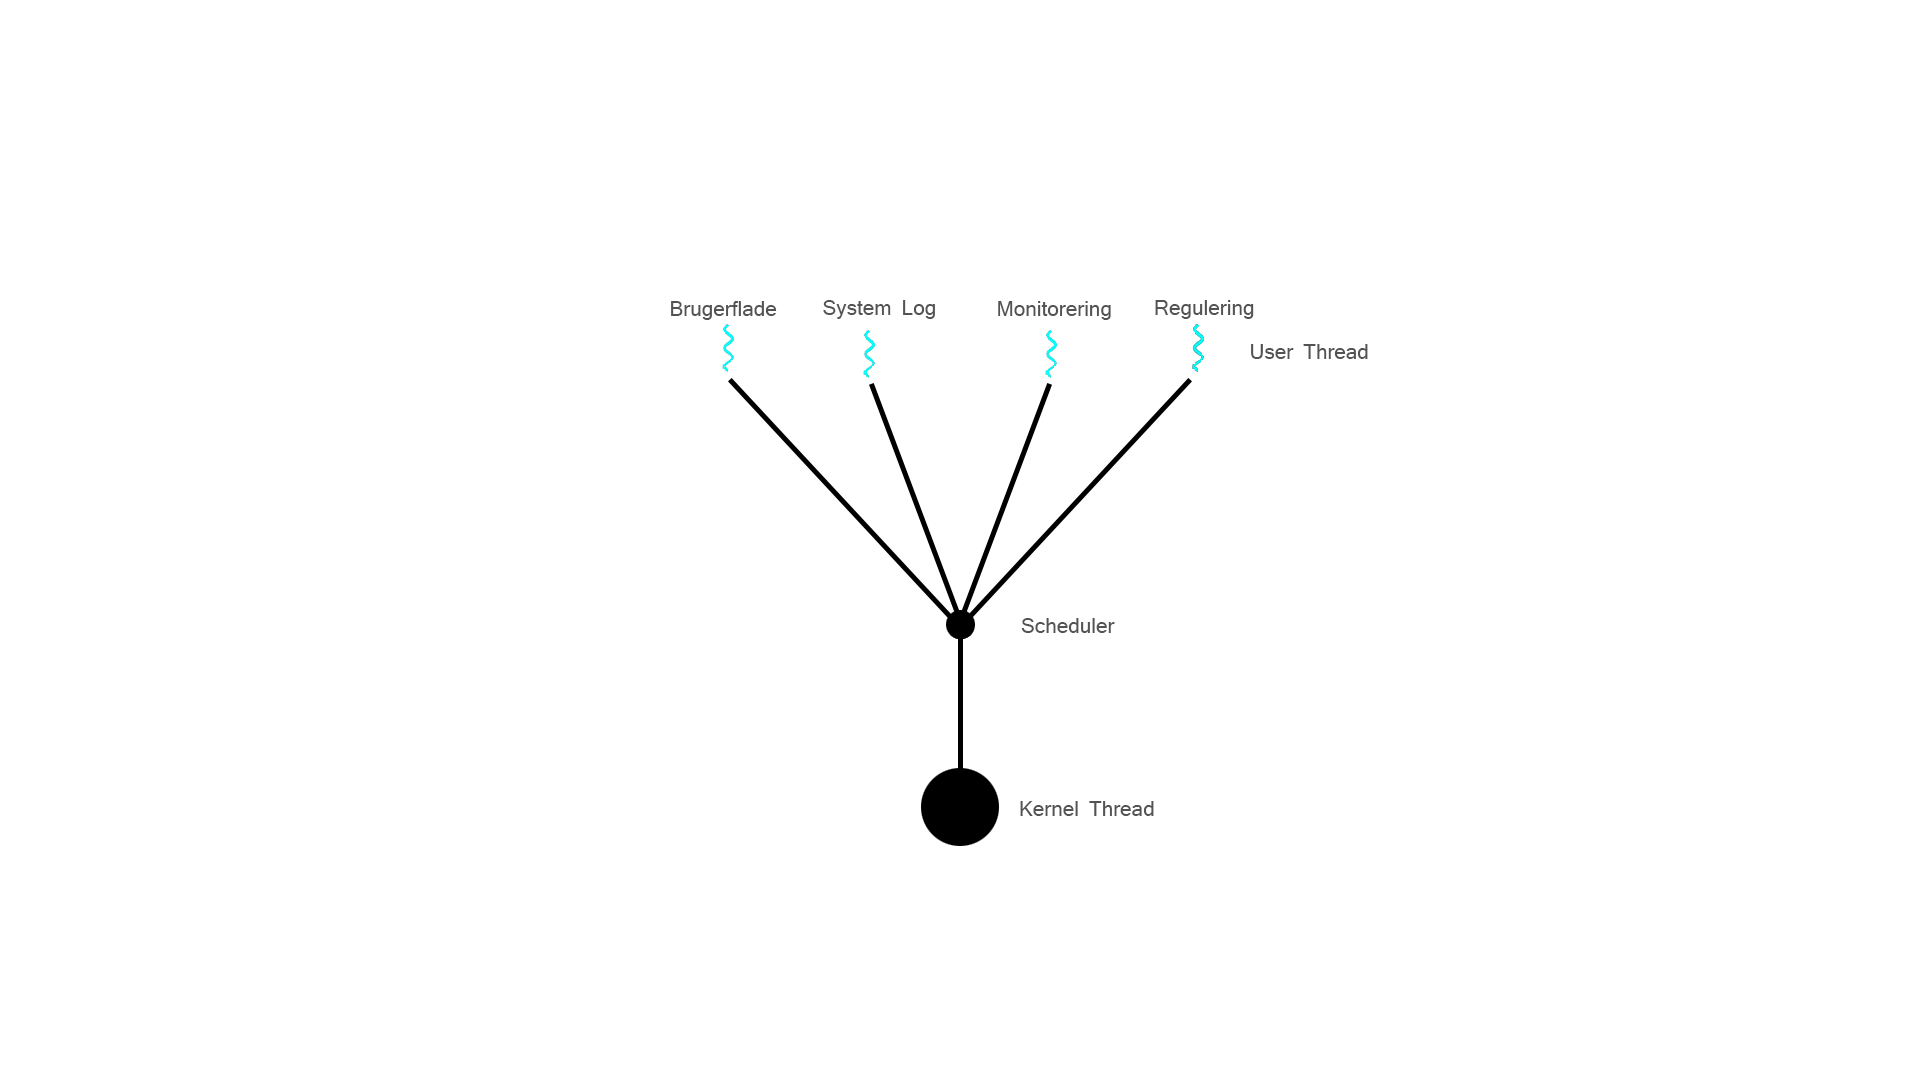
\includegraphics[width={\textwidth-2cm}, trim=600 200 550 250, clip=true] {../fig/Threads.png}
\caption{Thread opsætning af systemet}
\label{fig:SD_Threads}
\end{figure}